\section{懶人標記}
    \subsection{概念}
    之前的線段樹只有單點修改的功能,而若需要區間加值的話則會很費時,
    因此有人想到一個方法:若要修改的區間剛好完全包含線段樹上的某個區間的話,
    就可以先在上面打一個標記。等到需要動到他下面的子區間再向下放,
    因為我們一次最多在$O(\log n)$個區間打上標記,
    所以區間修改也可以從 $O(n\log(n))$ 進步到 $O(\log(n))$ 。

    \subsection{實作}
    首先我們需要在node裡面增加一些東西,因為標記稱為Tag,所以以下程式碼中
    的tag表示我們的標記。

\begin{lstlisting}[caption=懶人標記的node]
struct node{
    // value 和 tag
    int val,tag;

    // 子樹的指標
    node *rch,*lch;
    
    // 建構式
    node(){
        val=tag=0;
        rch=lch=nullptr;
    }

    // 帶有初始值的建構式
    node(int v){
        val=v, tag=0;
        rch=lch=nullptr;
    }
};
\end{lstlisting}

    接著,我們的node裡面會有一些函式,我以區間加值(將一段區間
    都加上某個數)為例。

\begin{lstlisting}[caption=懶人標記的node]
struct node{
    // 單點修改
    void modify(int p,int v,int lb=1,int rb=n){
        // 終止條件:區間長度為1
        if(lb==rb){
            val=v;
            return;
        }

        // 若左右子樹沒有結點則開一個新的
        if(!lch) lch=new node();
        if(!rch) rch=new node();

        push(lb,rb);
        
        // 設mid為區間中點,均分為左右區間
        // >>1相當於/2,但快很多
        int mid=lb+rb>>1;

        if(p<=mid) lch->modify(p,v, lb ,mid);
        if(mid<p)  rch->modify(p,v,mid+1,rb);

        // 還記得子樹修改完要做什麼?
        pull();
    }

    int query(int l,int r,int lb=1,int rb=n){
        if(l<=lb && rb<=r){
            return val;
        }

        push(lb,rb);
        
        int mid=lb+rb>>1;

        int ret=0;
        if(lch && l<=mid) ret+=lch->query(l,r, lb ,mid);
        if(rch && mid<r)  ret+=rch->query(l,r,mid+1,rb);

        pull();

        return ret;
    }
    
    // 區間加值
    void add(int l,int r,int v,int lb=1,int rb=n){
        // 終止條件:所在區間位於欲查詢區間之中
        if(l<=lb && rb<=r){
            // 由於區間為閉區間[lb,rb]因此要加1
            val+=v*(rb-lb+1);
            tag+=v;
            return;
        }

        push(lb,rb);
        
        int mid=lb+rb>>1;

        int ret=0;
        if(lch && l<=mid) lch->add(l,r,v, lb ,mid);
        if(rch && mid<r)  rch->add(l,r,v,mid+1,rb);

        pull();
    }
};
\end{lstlisting}

    另一種方式是用陣列,我們可以另外開一個陣列稱為tag。具體的程式
    架構與上述的指標型線段樹大致相同,就留給各位自行練習了。

    \subsection{範例與練習}
    \example TIOJ 1224 矩形覆蓋面積計算

    \textbf{題目敘述}

    給你很多平面上的矩形,請求出它們覆蓋的總表面積。

    \textbf{輸入說明}

    輸入檔案只包含一筆測試資料。

    第一行包含一個正整數 $n$,表示矩形的數量 ($1 \leq n \leq 100,000$)。

    接下來的 $n$ 行,每行包含四個整數 $L, R, D, U$ ($0 \leq L < R \leq 1,000,000$;$0 \leq D < U \leq 1,000,000$),
    代表矩形的左、右、下、上四個邊界座標。

    \textbf{輸出說明}

    請輸出覆蓋的總面積。

    \textbf{範例測試}

    \begin{tabular}{|m{7cm}|m{7cm}|}
        \hline
        範例輸入 1 & 範例輸出 1 \\
        \hline
        \verb|2|  & \verb|84| \\
        \verb|1 10 1 10|  & \\
        \verb|0 2 0 2|  &\\
        \hline
    \end{tabular}

    \textbf{想法}

    想像有一條線從上往下(或從下往上)掃描,每個矩形的上邊表示進入,
    下邊表示出來,我們可以藉由維護這個區間有多少地方是有被矩形覆蓋的
    直到有所變化(進或出),這所有區間長度總和,乘上上次有變化到這次有變化前高度
    就是這一段的面積。

    \begin{figure}[!htbp]
        \centering
        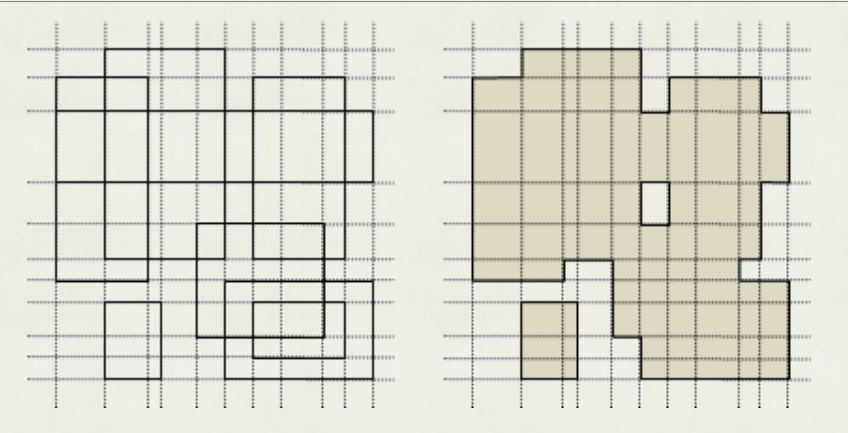
\includegraphics[width=0.8\textwidth]{../Images/LazyTag1.png}
        \caption{矩形覆蓋面積示意圖}
    \end{figure}

    \begin{figure}[!htbp]
        \centering
        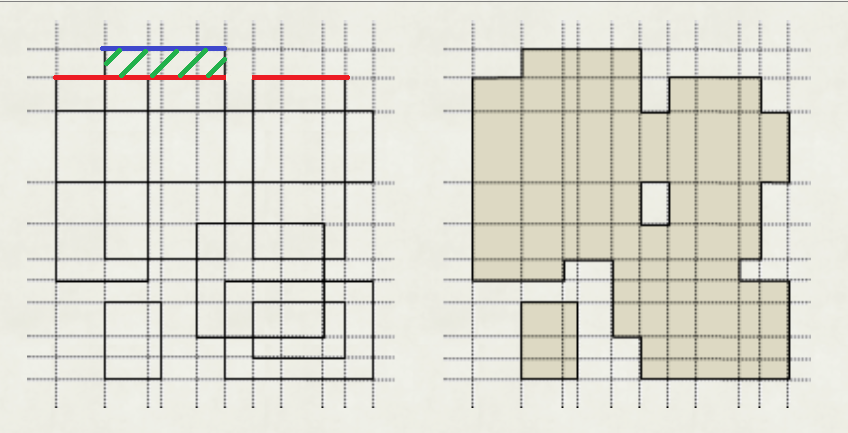
\includegraphics[width=0.8\textwidth]{../Images/LazyTag2.png}
        \caption{第一個變化}
    \end{figure}

    \begin{figure}[!htbp]
        \centering
        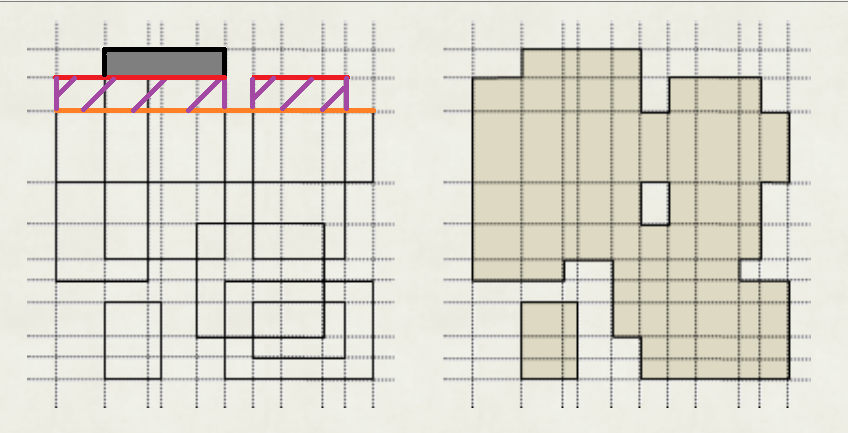
\includegraphics[width=0.8\textwidth]{../Images/LazyTag3.png}
        \caption{第二個變化}
    \end{figure}

    \textbf{實作}

    首先,我們需要一棵可以區間加值的線段樹。接著對所有的變化做排序,
    最後一一計算分部的面積。因為這題比較特殊,所以我貼上完整的程式碼。

    注意:因為我們只要查詢所有的和,所以我們可以使用跟節點的值就好。

\begin{lstlisting}[caption=矩形覆蓋面積題解]
#include<bits/stdc++.h>
using namespace std;

struct node{
    int ct=0,sum=0;
}seg[3050000];

struct line{
    int l,r,x,m;
    line(){
        l=r=x=0;
    }
    line(int a,int b,int c,int i){
        l=a;r=b;x=c;m=i;
    }
};
bool operator<(line a,line b){
    return a.x<b.x;
}

int n,MXN;
vector<line> lns;

void pull(int idx){
    seg[idx].sum=seg[idx*2].sum+seg[idx*2+1].sum;
}

void init(){
    MXN=1;
    while(MXN<1000010)
        MXN<<=1;
}

void add(int l,int r,int v,int lb=1,int rb=MXN,int idx=1){
    if(l<=lb && rb<=r){
        seg[idx].ct+=v;
        if(seg[idx].ct>0) seg[idx].sum=rb-lb+1;
        else pull(idx);
        return;
    }

    int mid=lb+rb>>1;
    if(l<=mid) add(l,r,v,lb,mid,idx*2);
    if(mid+1<=r) add(l,r,v,mid+1,rb,idx*2+1);
    
    if(seg[idx].ct>0) seg[idx].sum=rb-lb+1;
    else pull(idx);
}

int main(){
    ios::sync_with_stdio(0);cin.tie(0);
    
    cin>>n;
    for(int i=0;i<n;++i){
        int l,r,d,u;
        cin>>l>>r>>d>>u;
        lns.emplace_back(line(l+1,r,d,1));
        lns.emplace_back(line(l+1,r,u,-1));
    }
    sort(lns.begin(),lns.end());
    init();

    long long sum=0,pre=lns.front().x;
    for(auto ln:lns){
        if(ln.x != pre){
            sum+=(seg[1].sum)*(ln.x-pre);
            pre=ln.x;
        }
        add(ln.l,ln.r,ln.m);
    }
    sum+=(seg[1].sum)*(lns.back().x-pre);

    cout<<sum;
}
\end{lstlisting}

    \problem 洛谷P3870 【TJOI2009】開關

    \textbf{題目敘述}

    現有 $n$ 盞燈排成一排,從左到右依次編號為 $1$,$2$,……,$n$。然後依次執行 $m$ 項操作。

    操作分為兩種:
    \begin{enumerate}
        \item 指定一個區間 $[a,b]$,然後改變編號在這個區間內的燈的狀態(把開著的燈關上,關著的燈打開)。
        \item 指定一個區間 $[a,b]$,要求你輸出這個區間內有多少盞燈是打開的。
    \end{enumerate}
    
    燈在初始時都是關著的。

    \textbf{輸入說明}

    第一行有兩個整數 $n$ 和 $m$,分別表示燈的數目和操作的數目。

    接下來有 $m$ 行,每行有三個整數,依次為:$c$、$a$、$b$。其中 $c$ 表示操作的種類。

    \begin{enumerate}
        \item 當 $c$ 的值為 $0$ 時,表示是第一種操作。
        \item 當 $c$ 的值為 $1$ 時,表示是第二種操作。
    \end{enumerate}

    $a$ 和 $b$ 則分別表示了操作區間的左右邊界。

    $2\le n\le 10^5$,$1\le m\le 10^5$,$1\le a,b\le n$,$c\in \{0,1\}$

    \textbf{輸出說明}

    每當遇到第二種操作時,輸出一行,包含一個整數,表示此時在查詢的區間中打開的燈的數目。

    \textbf{範例測試}

    \begin{tabular}{|m{7cm}|m{7cm}|}
        \hline
        範例輸入 1 & 範例輸出 1 \\
        \hline
        \verb|4 5|  & \verb|1| \\
        \verb|0 1 2|  & \verb|2| \\
        \verb|0 2 4|  & \\
        \verb|1 2 3|  &\\
        \verb|0 2 4|  & \\
        \verb|1 1 4|  &\\
        \hline
    \end{tabular}

    \problem 洛谷P1438 無聊的數列

    \textbf{題目敘述}

    無聊的 YYB 總喜歡搞出一些正常人無法搞出的東西。有一天,無聊的 YYB 想出了一道無聊的題:無聊的數列。。。(K峰:這題不是傻X題嗎)

    維護一個數列 $a_i$,支持兩種操作:

    \verb|1 l r K D|:給出一個長度等於 $r-l+1$ 的等差數列,
    首項為 $K$,公差為 $D$,並將它對應加到 $[l,r]$ 範圍中的每一個數上。
    即:令 $a_l=a_l+K,a_{l+1}=a_{l+1}+K+D\ldots a_r=a_r+K+(r-l) \times D$。

    \verb|2 p|:詢問序列的第 $p$ 個數的值 $a_p$。

    \textbf{輸入說明}

    第一行兩個整數數 $n,m$ 表示數列長度和操作個數。

    第二行 $n$ 個整數,第 $i$ 個數表示 $a_i$。

    接下來的 $m$ 行,每行先輸入一個整數 $opt$。

    若 $opt=1$ 則再輸入四個整數 $l\ r\ K\ D$;

    若 $opt=2$ 則再輸入一個整數 $p$。

    $0\le n,m \le 10^5,-200\le a_i,K,D\le 200, 1 \leq l \leq r \leq n, 1 \leq p \leq n$

    \textbf{輸出說明}

    對於每個詢問,一行一個整數表示答案。

    \textbf{範例測試}

    \begin{tabular}{|m{7cm}|m{7cm}|}
        \hline
        範例輸入 1 & 範例輸出 1 \\
        \hline
        \verb|5 2|  & \verb|6| \\
        \verb|1 2 3 4 5|  & \\
        \verb|1 2 4 1 2|  & \\
        \verb|2 3|  &\\
        \hline
    \end{tabular}

    